\documentclass[12pt,compress,english,utf8,t]{beamer}
\usepackage[english]{babel}
\usepackage{calc}
\usepackage{ragged2e,wasysym,multicol,mathtools}
\usepackage[protrusion=true,expansion=true]{microtype}
\usepackage{tikz,ifthen}
\usetikzlibrary{calc,shapes,shapes.callouts,shapes.arrows,patterns,fit,backgrounds,decorations.pathmorphing}
\usepackage{booktabs}
\hypersetup{colorlinks=true}

\graphicspath{{images/}}

\title{Large numbers, very large numbers and very very large numbers}
\author{Ingo Blechschmidt and Matthias Hutzler}
\date{December 30th, 2018}

%\usetheme{Warsaw}
\useinnertheme[shadow=true]{rounded}
\useoutertheme{split}
\usecolortheme{orchid}
\usecolortheme{whale}
\setbeamerfont{block title}{size={}}

\useinnertheme{rectangles}

\usecolortheme{seahorse}
\definecolor{mypurple}{RGB}{150,0,255}
\setbeamercolor{structure}{fg=mypurple}
\definecolor{myred}{RGB}{150,0,0}
\setbeamercolor*{title}{bg=myred,fg=white}
\setbeamercolor*{titlelike}{bg=myred,fg=white}

\usefonttheme{serif}
\usepackage[T1]{fontenc}
\usepackage{libertine}

\renewcommand{\_}{\mathpunct{.}\,}
\newcommand{\BB}{\mathbb{B}}
\newcommand{\M}{\mathcal{M}}
\newcommand{\R}{\mathrm{R}}
\newcommand{\NN}{\mathbb{N}}
\newcommand{\RR}{\mathbb{R}}

\newcommand{\imgslide}[1]{{\usebackgroundtemplate{\parbox[c][\paperheight][c]{\paperwidth}{\centering\includegraphics[width=\paperwidth]{#1}}}\begin{frame}[plain]\end{frame}}}

\setbeamertemplate{navigation symbols}{}

\setbeamertemplate{title page}[default][colsep=-1bp,rounded=false,shadow=false]
\setbeamertemplate{frametitle}[default][colsep=-2bp,rounded=false,shadow=false,center]

\newcommand{\hil}[1]{{\usebeamercolor[fg]{item}{\textbf{#1}}}}
\setbeamertemplate{frametitle}{%
  \vskip1em%
  \leavevmode%
  \begin{beamercolorbox}[dp=1ex,center]{}%
      \usebeamercolor[fg]{item}{\textbf{\textsf{\Large \insertframetitle}}}
  \end{beamercolorbox}%
}

\setbeamertemplate{footline}{%
  \leavevmode%
  \hfill%
  \begin{beamercolorbox}[ht=2.25ex,dp=1ex,right]{}%
    \usebeamerfont{date in head/foot}
    \insertframenumber\,/\,\inserttotalframenumber\hspace*{1ex}
  \end{beamercolorbox}%
  \vskip0pt%
}

\newcommand{\backupstart}{
  \newcounter{framenumberpreappendix}
  \setcounter{framenumberpreappendix}{\value{framenumber}}
}
\newcommand{\backupend}{
  \addtocounter{framenumberpreappendix}{-\value{framenumber}}
  \addtocounter{framenumber}{\value{framenumberpreappendix}}
}

\setbeameroption{show notes}
\setbeamertemplate{note page}[plain]

% Taken from Todd Lehman (CC-BY-SA) at https://tex.stackexchange.com/a/44920/32372

\newcommand{\setisprime}[1]{
  % Sets \isprime based on #1.
  \ifnum#1=1 \gdef\isprime{0} \else \gdef\isprime{1} \fi
  \foreach \sip in {2, 3,5,...,#1} {
    \pgfmathparse{\sip*\sip>#1? 1:0}
    \ifthenelse{\pgfmathresult=1}{
      % Early-out if \sip^2 > #1.
      \breakforeach
    }{
      % Otherwise test if \sip divides #1.
      \pgfmathparse{Mod(#1,\sip)==0? 1:0}
      \ifthenelse{\pgfmathresult=1}{
        \gdef\isprime{0}
        \breakforeach
      }{}
    }
  }
}

\newcommand{\setxy}[1]{
  % Sets \x and \y to loction of cell #1.
  \pgfmathtruncatemacro{\x}{Mod(#1-1,\cols)}
  \pgfmathtruncatemacro{\y}{(#1-1) / \cols}
  \pgfmathtruncatemacro{\y}{\cols - 1 - \y}
  \pgfmathparse{2.5*(\x+.5)}\let\x\pgfmathresult
  \pgfmathparse{2.5*(\y+.5)}\let\y\pgfmathresult
}

\newcommand{\numlabel}[2]{
  % Draws label #2 at cell #1.
  \setxy{\n}
  \node[fill=none, text=black] at (\x,\y) {#2};
}

\newcommand{\drawpolygon}[2]{
  % Draws polygon with #2 vertexes at cell #1.
  \setxy{#1}
  \ifthenelse{#2>1}{ % Polygon must have at least 2 sides.
    \ifthenelse{#2<30}{ % Draw polygon if it has a small number of sides.
      \filldraw (\x,\y) +(90:1)
      \foreach \drawi in {1,...,#2} {-- +(\drawi/#2*360+90:1)} -- cycle;
    }{ % Else approximate with circle.
      \filldraw (\x,\y) circle(1);
    }
  }{}
}

\newcommand{\setpolygoncolor}[1]{
  % Sets color based on #1.
  \gdef\polycolor{black}
  \ifnum#1=2\gdef\polycolor{black!50!white}\fi
  \ifnum#1=3\gdef\polycolor{yellow!95!red}\fi
  \ifnum#1=5\gdef\polycolor{yellow!0!red}\fi
  \ifnum#1=7\gdef\polycolor{blue!75!green}\fi
  \ifnum#1=11\gdef\polycolor{blue!70!red}\fi
  \ifnum#1=13\gdef\polycolor{blue!40!red}\fi
  \ifnum#1=17\gdef\polycolor{green!50!blue}\fi
  \ifnum#1=19\gdef\polycolor{green!80!black}\fi
  \ifnum#1=23\gdef\polycolor{green!50!red}\fi
  \ifnum#1=29\gdef\polycolor{yellow!50!black}\fi
  \ifnum#1=31\gdef\polycolor{orange!50!black}\fi
  \ifnum#1=37\gdef\polycolor{red!50!black}\fi
  \ifnum#1=41\gdef\polycolor{purple!50!black}\fi
  \ifnum#1=43\gdef\polycolor{blue!50!black}\fi
  \ifnum#1=47\gdef\polycolor{green!50!black}\fi
  \ifnum#1=53\gdef\polycolor{white!50!black}\fi
  \ifnum#1=59\gdef\polycolor{white!50!black}\fi
  \ifnum#1=61\gdef\polycolor{white!50!black}\fi
  \ifnum#1=67\gdef\polycolor{white!50!black}\fi
}

\newcommand{\sieve}[2]{
  \def\cols{#1}
  \def\rows{#2}
  \begin{tikzpicture}[scale=.5,anchor=center]
  \pgfmathtruncatemacro{\nmax}{\rows * \cols}

  \foreach \n in {1,...,\nmax} {
    \begin{scope}[fill=gray, fill opacity=.05,
                  draw=gray, draw opacity=.10,
                  line width=4]
      \drawpolygon{\n}{\n}
    \end{scope}
    \setisprime{\n}
    \ifthenelse{\isprime=1}{
      \numlabel{\n}{\bf\n}
    }{
      \def\startintensity{.33}
      \def\incrintensity{.10}
      \def\intensity{\startintensity}

      \def\m{\n}
      \pgfmathtruncatemacro{\i}{\m / 2}

      % Divide \m by \i until \m is extinguished.
      % Increment \i each time it does not divide into \m.
      \whiledo{\m>1}{
        \setisprime{\i}
        \pgfmathparse{Mod(\m,\i)==0? 1:0}
        \ifthenelse{\pgfmathresult=1\and\isprime=1}{
          \setpolygoncolor{\i}
          \begin{scope}[fill=\polycolor, fill opacity=\intensity,
                        draw=\polycolor!85!black, draw opacity=\intensity,
                        line width=\intensity*1.5]
            \drawpolygon{\n}{\i}
          \end{scope}
          \pgfmathtruncatemacro{\m}{\m / \i}
          \pgfmathparse{\intensity + \incrintensity}\let\intensity\pgfmathresult
        }{
          \pgfmathtruncatemacro{\i}{\i - 1}
          \def\intensity{\startintensity}
        }
      }
      \begin{scope}[text=black, text opacity=.5]
        \numlabel{\n}{\scriptsize\n}
      \end{scope}
    }
  }

  \end{tikzpicture}
}


\setbeamertemplate{headline}{
  \begin{beamercolorbox}[wd=\paperwidth,ht=2.25ex]{}%
    foo
  \end{beamercolorbox}
}

\addtocounter{framenumber}{-1}

\begin{document}

{\usebackgroundtemplate{\begin{minipage}{\paperwidth}\vspace*{0.3cm}\centering\scriptsize\sieve{25}{2}\\\vspace*{3.95cm}\includegraphics[width=\paperwidth]{sun3}\end{minipage}}
\begin{frame}[c]
  \centering

  \bigskip
  \bigskip
  \bigskip
  \bigskip
  \bigskip

  \hil{Large numbers,}
  
  \large
  \hil{very large numbers,}
  
  \Large
  \hil{very very large numbers}

  \bigskip
  \scriptsize
  \textit{-- an invitation to advanced goology --}
  \bigskip
  \bigskip
  \bigskip
  \bigskip
  \medskip

  \begin{minipage}{4cm}
    \centering
    \textcolor{white}{
      Ingo Blechschmidt \\
      Università di Verona
    }
  \end{minipage}
  \begin{minipage}{4cm}
    \centering
    \textcolor{white}{
      Matthias Hutzler \\
      Universität Augsburg
    }
  \end{minipage}

  \bigskip

  \textcolor{white}{
    35th Chaos Communication Congress \\
    December 30th, 2018
  }
  \par
\end{frame}}


\section{Large numbers}

\tikzstyle{card}   = [draw=mypurple, very thick, rectangle, rounded corners, inner sep=5pt, inner ysep=10pt]
\tikzstyle{author} = [fill=mypurple, text=white]
\tikzstyle{descr}  = []

\newcommand{\card}[2]{
  \begin{tikzpicture}
    \node[descr]  (descr)  {#2};
    \node[card, tape] [fit = (descr)] (card) {};
    \node[author] at (card.north) (author) {#1};
  \end{tikzpicture}
}

{\usebackgroundtemplate{\begin{minipage}{\paperwidth}\vspace*{6.5cm}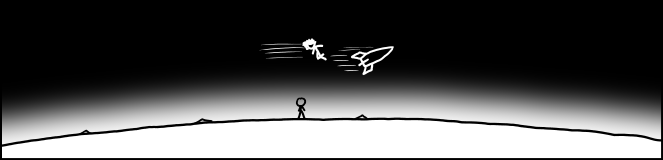
\includegraphics[width=\paperwidth]{sandkoerner}\end{minipage}}
\begin{frame}
  \centering
  \bigskip

  \Huge \hil{Part 0}

  \bigskip
  \Large\textbf{Large numbers}
  \par
  \bigskip

  \normalsize

  \hil{15\,000} congress participants
  \medskip

  \hil{1234} grains of sand on earth
  \medskip

  \hil{$\boldsymbol{10^{80} = 1\!\underbrace{000\ldots000}_{\text{$80$ zeros}}}$}
  elementary particles in the universe

  % VIDEO: mass of black hole
\end{frame}}

\begin{frame}
  \card{foo}{$9\!\underbrace{!!!!!!!\ldots!!!!!!!}_{\text{4095 factorials}}$}
\end{frame}

\end{document}

{\usebackgroundtemplate{\begin{minipage}{\paperwidth}\hfill\includegraphics[height=\paperheight]{images/orbit-tall}\end{minipage}}
\begin{frame}{Basic facts}
  \begin{itemize}
    \item Getting to space is easy. \\ The hard part is staying there.
    \item Gravitational acceleration at \\ the height of the ISS is still $\approx 8.7 \,\mathrm{m}/\mathrm{s}^2$.
    % Mention: no friction.
  \end{itemize}
\end{frame}}


\subsection{Basic facts}

\begin{frame}{Basic facts}
  \begin{itemize}
    \item<1-> Getting to space is easy. \\ The hard part is staying there.
    \item<3-> Velocity is very important.
    \item<4-> In the \hil{one-body problem}, there are only three kinds of
    orbits: elliptic, parabolic, and hyperbolic.
    \item<5-> Have your models straight: Earth is \ldots
    \begin{enumerate}
      \item a perfect ball?
      \item has atmosphere?
      \item rotating?
    \end{enumerate}
    % instantaneous impulses?
  \end{itemize}

  \only<1>{
    \centering
    % https://upload.wikimedia.org/wikipedia/commons/thumb/7/73/Newton_Cannon.svg/240px-Newton_Cannon.svg.png
    \vspace*{-7em}
    \includegraphics[width=0.4\textwidth]{images/newton-cannon}

    $F_{\text{centripetal}} = F_{\text{gravitation}}
    \leadsto v_1 = \sqrt{GM/r}$

    $E_{\text{kinetic}} = E_{\text{gravitation}}
    \leadsto v_2 = \sqrt{2} \, v_1$
    \par
  }

  \only<2>{
    \centering
    \vspace*{-4em}
    \begin{tabular}{ll}
      \toprule
      body & second escape velocity \\\midrule
      Earth & $11.2 \,\mathrm{km}/\mathrm{s} \approx 40\,000 \,\mathrm{km}/\mathrm{h}$ \\
      Moon  & $2.4  \,\mathrm{km}/\mathrm{s}$ \\
      Sun   & $618  \,\mathrm{km}/\mathrm{s}$ \\
      Milky Way & $\approx 550 \,\mathrm{km}/\mathrm{s}$ \\
      \bottomrule
    \end{tabular}
    \par
  }
\end{frame}


\subsection[Changing orbits]{Changing orbits}

\begin{frame}{Changing orbits}
  \begin{center}
    \hil{``Live demo''}
  \end{center}

  \begin{itemize}
    \item Changing the phase

    % Winkel ändern:
    % Speed away from the central body.
    % Necessary Δv depends on eccentricity.
    % If eccentricity is zero, need to Δv.

    \item Changing the eccentricity
    % Accelerate in tangential direction

    \item Changing the radius
    % Hohmann transfer

    \item Changing inclination
    % Easy, just accelerate normal to the plane.
  \end{itemize}
\end{frame}

\imgslide{clips/02-chinese-space-station}


\subsection[Rocket equation]{The tyranny of the rocket equation}

\begin{frame}{The tyranny of the rocket equation}
  \centering
  % http://tsiolkovsky.org/wp-content/uploads/2015/02/icon_en.png
  \includegraphics[width=0.4\textwidth]{images/tsiolkovsky} \\
  {\scriptsize Konstantin Tsiolkovsky (* 1857, † 1935)\par}
  \bigskip

  \scalebox{2}{$m_\text{total} = m_\text{payload} \cdot e^{\Delta v / v_\text{eff.\@ exhaust}}$}
  \par
\end{frame}

% Weltall ist nah.
% Extrem wichtig: (Ort,Geschwindigkeit) des Ziels
% Erste Fluchtgeschwindigkeit
% Filmausschnitt Bruce Willis
% Filmausschnitt Gravity?
% Arten von Trajektorien (stets Ellipsen, Parabeln oder Hyperbeln)
% Tyrannei der Raketengleichung
% Orbitwechsel
% Gravity assist


\section[Chaos theory]{One weird trick from chaos theory}

{\usebackgroundtemplate{\includegraphics[height=\paperheight]{images/Interplanetary_Superhighway}}
\begin{frame}
  \centering
  \bigskip\bigskip

  \Huge \hil{Part II}

  \bigskip
  \Large\textcolor{white}{\textbf{One weird trick from chaos theory}}
  \par
\end{frame}}


\subsection{Lagrangian points}

\begin{frame}{Lagrangian points}
  \centering
  \only<1>{\includegraphics[width=0.7\textwidth]{lagrange}}
  \only<2>{\includegraphics[width=0.7\textwidth]{lagrange2}}
  \par
\end{frame}


\subsection{Weak stability boundaries}

\begin{frame}{Weak stability boundaries}
  \centering
  \only<1>{\includegraphics[width=0.6\textwidth]{weak-stability-boundaries}}
  \only<2>{\includegraphics[width=0.7\textwidth]{weak-stability-boundary-plot}}
  \par
\end{frame}

\imgslide{clips/03-supercomputer-1}


\subsection[Hiten]{The rescue of the Hiten}

\begin{frame}{The rescue of the Hiten}
  \centering
  \includegraphics[width=0.7\textwidth]{hiten-trajectory}
  \par
\end{frame}


\subsection{In nature}

\begin{frame}{In nature}
  \centering
  \includegraphics[width=0.6\textwidth]{intergalactic-transport-network}
  \par
\end{frame}

% https://upload.wikimedia.org/wikipedia/commons/thumb/7/78/L4_diagram.svg/403px-L4_diagram.svg.png
% https://upload.wikimedia.org/wikipedia/commons/5/5f/Lagrangian_points_equipotential.jpg

% Zunächst: Orbiten komplizierter!
% Probleme mit konventionellem Ansatz (auch Neustartprobleme)
% Ziel: ballistisches Einfangen
% Lagrange-Punkte (Krassheit der Punkte nicht vergessen)
% dazu mitrotierendes Bezugssystem, Zentrifugalkraft, Corioliskraft
% WSM
% Wie man sie findet
% Hiten
% In der Natur

% Wurmlochnostalgie nicht vergessen!
% Krasse Rundtourtrajektorien nicht vergessen!
% Szene aus The Martian nicht vergessen!
% Szene aus Gravity nicht vergessen!
% Swing-by-Manöveur nicht vergessen!
% Hohmann-Transfer nicht vergessen!
% Krasse Stärke der Gravitation beiläufig erwähnen.

\end{document}
